\addcontentsline{toc}{section}{Introduction}
\section*{Introduction}


Data warehouses and data lakes are the most common central data repositories employed by most data-driven organizations today, each with its own strengths and tradeoffs. For one, while data warehouses allow businesses to organize historical datasets for use in business intelligence (BI) and analytics, they quickly become more cost-intensive as datasets grow because of the combined use of compute and storage resources. Additionally, data warehouses can’t handle the varied nature of data (structured, unstructured, and semi-structured) seen today.

In this chapter, we will explore the key features of Delta Lake, how it works, and why it is a good choice for big data processing. We will also provide examples of how to use Delta Lake with other big data tools, such as Spark and Trino later on in this report.
\section{Definition}
Delta Lake is an open-source storage layer built atop a data lake that confers reliability and ACID (Atomicity, Consistency, Isolation, and Durability) transactions. It enables a continuous and simplified data architecture for organizations. A data lake stores data in Parquet formats and enables a lakehouse data architecture, which helps organizations achieve a single, continuous data system that combines the best features of both the data warehouse and data lake while supporting streaming and batch processing.

\section{How Delta Lake Works}
A Delta Lake enables the building of a data lakehouse. Common lakehouses include the Databricks Lakehouse and Azure Databricks. This continuous data architecture allows organizations to harness the benefits of data warehouses and data lakes with reduced management complexity and cost. Here are some ways Delta Lake improves the use of data warehouses and lakes:
\begin{itemize}
    \item \textbf{Enables a lakehouse architecture:} Delta Lake enables a continuous and simplified data architecture that allows organizations to handle and process massive volumes of streaming and batch data without the management and operational hassles involved in managing streaming, data warehouses, and data lakes separately.
    \item \textbf{Enables intelligent data management for data lakes:} Delta Lake offers efficient and scalable metadata handling, which provides information about the massive data volumes in data lakes. With this information, data governance and management tasks proceed more efficiently.
    \item \textbf{Schema enforcement for improved data quality:} Because data lakes lack a defined schema, it becomes easy for bad/incompatible data to enter data systems. There is improved data quality thanks to automatic schema validation, which validates DataFrame and table compatibility before writes.
    \item \textbf{Enables ACID transactions:} Most organizational data architectures involve a lot of ETL and ELT movement in and out of data storage, which opens it up to more complexity and failure at node entry points. Delta Lake ensures the durability and persistence of data during ETL and other data operations. Delta lake captures all changes made to data during data operations in a transaction log, thereby ensuring data integrity and reliability during data operations.
\end{itemize}

\section{Delta Lake Architecture Diagram}
\begin{flushleft}
Delta Lake is an improvement from the lambda architecture whereby streaming and batch processing occur parallel, and results merge to provide a query response. However, this method means more complexity and difficulty maintaining and operating both the streaming and batch processes. Unlike the lambda architecture, Delta Lake is a continuous data architecture that combines streaming and batch workflows in a shared file store through a connected pipeline.
\end{flushleft}

The stored data file has three layers, with the data getting more refined as it progresses downstream in the dataflow:

\begin{enumerate}
\item[$\bullet$] \textbf{Bronze tables:} This table contains the raw data ingested from multiple sources like the Internet of Things (IoT) systems, CRM, RDBMS, and JSON files.
\item[$\bullet$] \textbf{Silver tables:} This layer contains a more refined view of our data after undergoing transformation and feature engineering processes.
\item[$\bullet$] \textbf{Gold tables:} This final layer is often made available for end users in BI reporting and analysis or use in machine learning processes.
\end{enumerate}

\begin{figure}[htbp]
\centering
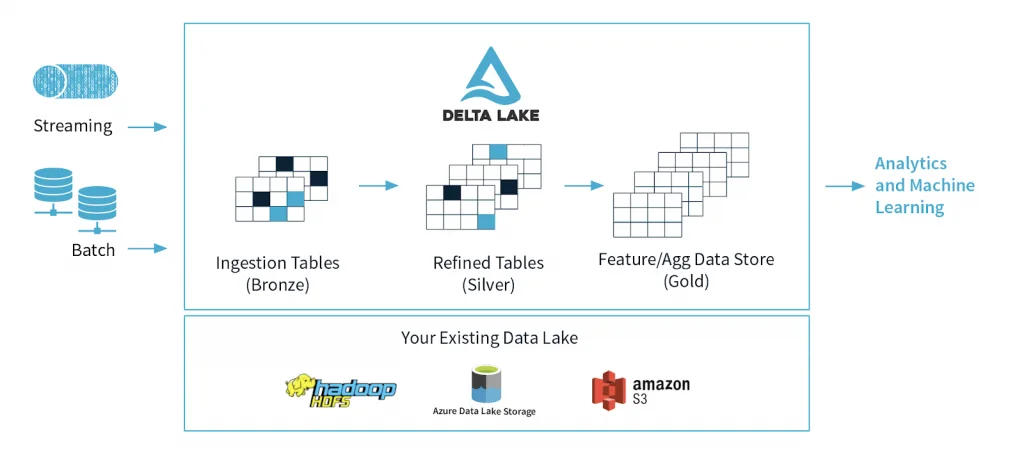
\includegraphics[width=\linewidth]{images/delta_lake_architecture.png}
\caption{Delta Lake multi-hop architecture}\label{fig:delta-lake-architecture}
\end{figure}

\section{Key benefits and features of Delta Lake}
\begin{itemize}
    \item[\textbullet] \textbf{Audit trails and history:} In Delta Lake, every write exists as a transaction and is serially recorded in a transaction log. Therefore, any changes or commits made to the transaction log are recorded, leaving a complete trail for use in historical audits, versioning, or for time traveling purposes. This Delta Lake feature helps ensure data integrity and reliability for business data operations.
    \item[\textbullet] \textbf{Time traveling and data versioning:} Because each write creates a new version and stores the older version in the transaction log, users can view/revert to older data versions by providing the timestamp or version number of an existing table or directory to the Sparks read API\@. Using the version number provided, the Delta Lake then constructs a full snapshot of the version with the information provided by the transaction log. Rollbacks and versioning play a vital role in machine learning experimentation, whereby data scientists iteratively change hyperparameters to train models and can revert to changes if needed.
    \item[\textbullet] \textbf{Unifies batch and stream processing:} Every table in a Delta Lake is a batch and streaming sink. With Sparks structured streaming, organizations can efficiently stream and process streaming data. Additionally, with the efficient metadata handling, ease of scale, and ACID quality of each transaction, near-real-time analytics become possible without utilizing a more complicated two-tiered data architecture.
    \item[\textbullet] \textbf{Efficient and scalable metadata handling:} Delta Lakes store metadata information in the transaction log and leverages Spark's distributed processing power to quickly process and efficiently read and handle large volumes of data metadata, thus improving data governance.
    \item[\textbullet] \textbf{ACID transactions:} Delta Lakes ensure that users always see a consistent data view in a table or directory. It guarantees this by capturing every change made in a transaction log and isolating it at the strongest isolation level, the serializable level. In the serializable level, every existing operation has and follows a serial sequence that, when executed one by one, provides the same result as seen in the table.
    \item[\textbullet] \textbf{Data Manipulation Language operations:} Delta Lakes supports DML operations like updates, deletes, and merges, which play a role in complex data operations like change-data-capture (CDC), streaming upserts, and slowly-changing-dimension (SCD). Operations like CDC ensure data synchronization in all data systems and minimizes the time and resources spent on ELT operations. For instance, using the CDC, instead of ETL-ing all the available data, only the recently updated data since the last operation undergoes a transformation.
    \item[\textbullet] \textbf{Schema enforcement:} Delta Lakes perform automatic schema validation by checking against a set of rules to determine the compatibility of a write from a DataFrame to a table. One such rule is the existence of all DataFrame columns in the target table. An occurrence of an extra or missing column in the DataFrame raises an exception error. Another rule is that the DataFrame and target table must contain the same column types, which otherwise will raise an exception. Delta Lake also use DDL (Data Definition Language) to add new columns explicitly. This data lake feature helps prevent the ingestion of incorrect data, thereby ensuring high data quality.
    \item[\textbullet] \textbf{Compatibility with Spark's API:} Delta Lake is built on Apache Spark and is fully compatible with Spark API, which helps build efficient and reliable big data pipelines.
    \item[\textbullet] \textbf{Flexibility and integration:} Delta lake is an open-source storage layer and utilizes the Parquet format to store data files, which promotes data sharing and makes it easier to integrate with other technologies and drive innovation.
\end{itemize}

\section{Implementation}
To use Delta Lake interactively within the Spark SQL, Scala, or Python shell, we need a local installation of Apache Spark. Depending on whether we want to use SQL, Python, or Scala, we can set up either the SQL, PySpark, or Spark shell, respectively.

\subsection*{Spark SQL Shell:}

\begin{lstlisting}[language=bash]
    bin/spark-sql --packages io.delta:delta-core_2.12:2.3.0
    --conf "spark.sql.extensions=io.delta.sql.DeltaSparkSessionExtension"
    --conf "spark.sql.catalog.spark_catalog=org.apache.spark.sql.delta.catalog.DeltaCatalog"
\end{lstlisting}

\subsection*{PySpark Shell:}
\begin{enumerate}
    \item Install the PySpark version that is compatible with the Delta Lake version by running the following:
    \begin{lstlisting}[language=bash]
    pip install pyspark==<compatible-spark-version>
    \end{lstlisting}
    \item Run PySpark with the Delta Lake package and additional configurations:
    \begin{lstlisting}[language=bash]
    pyspark --packages io.delta:delta-core_2.12:2.3.0 
    --conf "spark.sql.extensions=io.delta.sql.DeltaSparkSessionExtension" 
    --conf "spark.sql.catalog.spark_catalog=org.apache.spark.sql.delta.catalog.DeltaCatalog"
    \end{lstlisting}
\end{enumerate}

\subsection*{Scala Shell:}
Download the compatible version of Apache Spark by following instructions from Downloading Spark, either using pip or by downloading and extracting the archive and running spark-shell in the extracted directory.

\begin{lstlisting}[language=bash]
    bin/spark-shell --packages io.delta:delta-core_2.12:2.3.0 
    --conf "spark.sql.extensions=io.delta.sql.DeltaSparkSessionExtension" 
    --conf "spark.sql.catalog.spark_catalog=org.apache.spark.sql.delta.catalog.DeltaCatalog"
\end{lstlisting}

\subsection*{Create Table:}
To create a Delta table, write a DataFrame out in the delta format. We can use existing Spark SQL code and change the format from parquet, csv, json, and so on, to delta.

\begin{enumerate}
    \item \textbf{SQL:}
    \begin{lstlisting}[language=sql]
    CREATE TABLE delta.`/tmp/delta-table` USING DELTA AS SELECT col1 as id FROM VALUES 0,1,2,3,4;
    \end{lstlisting}
    \item \textbf{Python:}
    \begin{lstlisting}[language=python]
    data = spark.range(0, 5)
    data.write.format("delta").save("/tmp/delta-table")
    \end{lstlisting}
    \item \textbf{Scala:}
    \begin{lstlisting}[language=scala]
    val data = spark.range(0, 5)
    data.write.format("delta").save("/tmp/delta-table")
    \end{lstlisting}
    \item \textbf{Java:}
    \begin{lstlisting}[language=java]
    import org.apache.spark.sql.SparkSession;
    import org.apache.spark.sql.Dataset;
    import org.apache.spark.sql.Row;
    
    SparkSession spark = ...   // create SparkSession
    
    Dataset<Row> data = spark.range(0, 5);
    data.write().format("delta").save("/tmp/delta-table");
    \end{lstlisting}
\end{enumerate}

These operations create a new Delta table using the schema that was inferred from your DataFrame

\section*{Conclusion}
\addcontentsline{toc}{section}{Conclusion}

Delta Lake is an important tool for big data processing, providing reliable data management and ensuring data integrity at scale. Its ACID transactions, schema enforcement, and data versioning features make it a popular choice for companies that need to process large amounts of data with high accuracy and reliability.

By using Delta Lake, data engineers and data scientists can easily manage data quality, track data lineage, and collaborate on data analysis projects. With its seamless integration with other big data tools. Delta Lake provides a powerful solution for big data processing that can help companies gain insights from their data faster and more efficiently.
